\documentclass[11pt,a4paper]{article}
\usepackage[T1]{fontenc}
\usepackage[utf8]{inputenc}
\usepackage{lmodern}
\usepackage{textcomp}
\usepackage[left=1.8cm,right=1.8cm,top=3.0cm,bottom=2.2cm,headheight=36pt,headsep=12pt]{geometry}
\usepackage{multicol}
\usepackage{xcolor}
\usepackage{fancyhdr}\usepackage{tikz}
\usepackage{graphicx}
\usepackage{array}
\usepackage{amsmath,amssymb}
\usepackage{setspace}
\usepackage{longtable}
\graphicspath{{../}}
\definecolor{ygreen}{RGB}{46,139,87}\definecolor{dgreen}{RGB}{28,90,56}
\renewcommand{\normalsize}{\fontsize{10.9}{13.4}\selectfont}
\renewcommand{\familydefault}{\rmdefault}
\setlength{\parindent}{0pt}
\setlength{\columnsep}{0.8cm}
\setlength{\columnseprule}{0.4pt}
\setlength{\multicolsep}{3pt plus 1pt minus 1pt}
\renewcommand{\textsubscript}[1]{\ensuremath{_{\text{\fontsize{8}{8}\selectfont #1}}}}
\renewcommand{\textsuperscript}[1]{\ensuremath{^{\text{\fontsize{8}{8}\selectfont #1}}}}
\newcommand{\qn}[1]{\textbf{\fontsize{11.5}{13}\selectfont #1}}
\newcommand{\qsep}{\par\vspace{13pt}}
\newcommand{\fwrule}{\par\vspace{5pt}\noindent\rule{\linewidth}{1.4pt}\par\vspace{7pt}}
\newsavebox{\fitb}
\newcommand{\fitbox}[1]{\sbox{\fitb}{#1}\ifdim\wd\fitb>\linewidth\resizebox{\linewidth}{!}{\usebox{\fitb}}\else\usebox{\fitb}\fi}
\newcommand{\diqqat}[1]{\par\smallskip\noindent\textbf{Diqqat!} #1\par\medskip}
\newcommand{\javob}{\par\nopagebreak[4]\smallskip\noindent\textbf{Javob:} \rule[-2pt]{7.5cm}{0.4pt}\par\smallskip\noindent\textbf{Diqqat!} Javobingizni javoblar varaqasiga ko`chirib yozing.\par\medskip}
\pagestyle{fancy}
\fancyhf{}
\renewcommand{\headrulewidth}{1.6pt}\renewcommand{\headrule}{{\color{ygreen}\hrule height 1.6pt width\headwidth}}
\newcommand{\hdrlogo}{
\begin{tikzpicture}[baseline=0pt]\fill[ygreen,rounded corners=3pt] (0,0) rectangle (0.95,0.95);\node[white,font=\fontsize{24}{26}\bfseries\selectfont] at (0.475,0.47){K};\node[anchor=west,font=\fontsize{16}{18}\bfseries\selectfont,text=dgreen] at (1.15,0.66){KIMYO};\node[anchor=west,font=\footnotesize\scshape,text=gray] at (1.15,0.2){Milliy sertifikat\ \ 2026};\end{tikzpicture}}
\newcommand{\hdrpill}[1]{\begin{tikzpicture}[baseline=0pt]\node[fill=ygreen,text=white,rounded corners=8pt,inner xsep=10pt,inner ysep=5pt,font=\fontsize{13}{15}\bfseries\selectfont] at (0,0.475){#1};\end{tikzpicture}}
\fancyhead[L]{\hdrlogo}
\fancyhead[R]{\hdrpill{3-variant}}

\fancyfoot[C]{\thepage}
\fancypagestyle{first}{\fancyhf{}\renewcommand{\headrulewidth}{1.6pt}\renewcommand{\headrule}{{\color{ygreen}\hrule height 1.6pt width\headwidth}}\fancyhead[L]{\hdrlogo}\fancyhead[R]{\hdrpill{3-variant}}\fancyfoot[C]{\thepage}}
\begin{document}
\normalsize
\thispagestyle{first}
\noindent\textit{Davriy jadvaldan foydalanish mumkin.}
\par\smallskip
\begin{multicols}{2}
\noindent\qn{1.} Kislorod (\textit{Z} = 8) atomi elektron konfiguratsiyasida jami nechta juftlashgan elektron bor?

\noindent A)~\textsl{7} \hfill B)~\textsl{5} \hfill C)~\textsl{6} \hfill D)~\textsl{8}\par
\qsep
\noindent\qn{2.} Quyidagi zarrachalardan qaysilari argon atomi bilan izoelektron? 1) K\textsuperscript{+}; 2) Ca\textsuperscript{2+}; 3) N\textsuperscript{3$-$}; 4) Cl\textsuperscript{$-$}

\noindent A)~\textsl{1, 3} \hfill B)~\textsl{3, 4} \hfill C)~\textsl{1, 2, 4} \hfill D)~\textsl{2, 4}\par
\qsep
\noindent\qn{3.} K\textsubscript{2}CO\textsubscript{3} ning suvli eritmasi inert elektrodlar bilan elektroliz qilinganda qaysi moddalar ajraladi?

\noindent\begin{tabular}{@{}p{0.47\linewidth}@{}p{0.47\linewidth}@{}}
A)~\textsl{Ag va O\textsubscript{2}} & B)~\textsl{H\textsubscript{2} va O\textsubscript{2}} \\
C)~\textsl{Cu va Cl\textsubscript{2}} & D)~\textsl{H\textsubscript{2}, Cl\textsubscript{2} va NaOH} \\
\end{tabular}\par
\qsep
\noindent\qn{4.} P + HNO\textsubscript{3} + H\textsubscript{2}O $\to$ H\textsubscript{3}PO\textsubscript{4} + NO reaksiya tenglamasini tenglang va barcha koeffitsiyentlar \textbf{yig`indisini aniqlang.}

\noindent A)~\textsl{19} \hfill B)~\textsl{18} \hfill C)~\textsl{17} \hfill D)~\textsl{20}\par
\qsep
\noindent\qn{5.} pH = 2 bo`lgan HCl eritmasidan 101 ml va pH = 12 bo`lgan NaOH eritmasidan 99 ml aralashtirildi. Hosil bo`lgan eritmaning pH \textbf{ini aniqlang.}

\noindent A)~\textsl{4} \hfill B)~\textsl{5} \hfill C)~\textsl{3} \hfill D)~\textsl{7}\par
\qsep
\noindent\qn{6.} Grafikda A moddaning konsentratsiyasi vaqt bo`yicha o`zgarishi ko`rsatilgan.
\begin{center}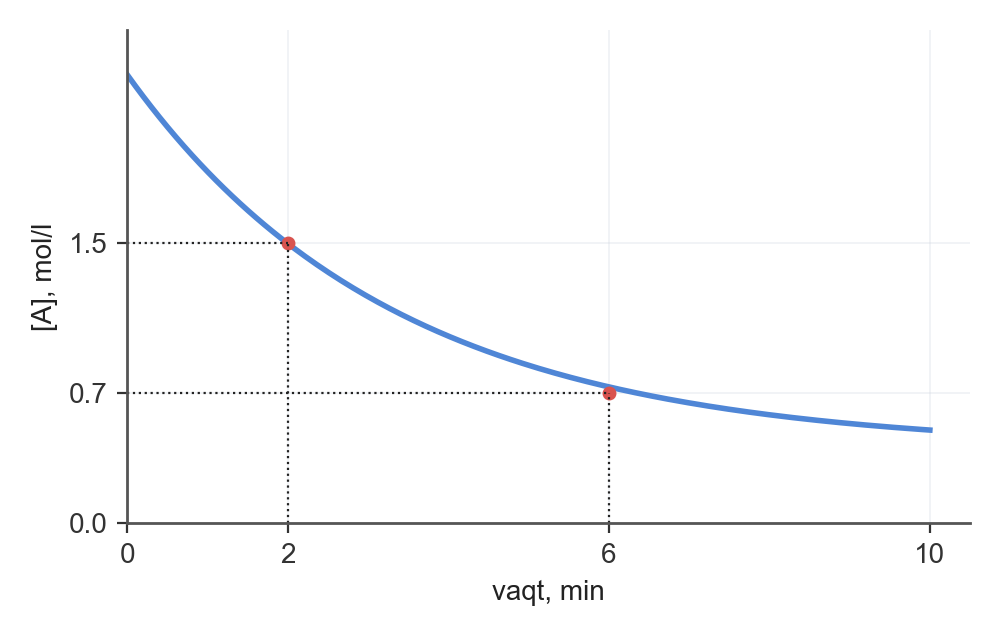
\includegraphics[width=0.86\linewidth]{rasmlar/gen/rate_v03_0.png}\end{center}
2-minutdagi A konsentratsiyasi 6-minutdagidan necha marta katta?

\noindent A)~\textsl{2,14} \hfill B)~\textsl{0,47} \hfill C)~\textsl{0,8} \hfill D)~\textsl{1,05}\par
\qsep
\noindent\qn{7.} 200 g CaCO\textsubscript{3} qizdirilganda uning 60\% i parchalandi. Qattiq qoldiq mo`l xlorid kislotada to`liq eritildi. Sarflangan HCl \textbf{massasini (g) aniqlang.}

\noindent A)~\textsl{87,6} \hfill B)~\textsl{58,4} \hfill C)~\textsl{146} \hfill D)~\textsl{292}\par
\qsep
\noindent\qn{8.} 2 mol C\textsubscript{2}H\textsubscript{6} va 1 mol CO\textsubscript{2} aralashmasidagi $\pi$-bog`lar umumiy \textbf{sonini (N\textsubscript{A} birligida) aniqlang.}

\noindent A)~\textsl{16} \hfill B)~\textsl{18} \hfill C)~\textsl{4} \hfill D)~\textsl{2}\par
\qsep
\noindent\qn{9.} 0,2 mol/l li sirka kislota eritmasining 5 l ida (dissotsilanish darajasi $\alpha$ = 0,05) suv molekulalaridan tashqari jami necha mol zarracha (molekula va ionlar) bor?

\noindent A)~\textsl{1} \hfill B)~\textsl{0,95} \hfill C)~\textsl{1,1} \hfill D)~\textsl{1,05}\par
\qsep
\noindent\qn{10.} 2SO\textsubscript{2} + O\textsubscript{2} $\rightleftarrows$ 2SO\textsubscript{3} reaksiyasi 2 l hajmli idishda o`tkazildi. Ma'lumotlar jadvalda berilgan:
\begin{center}
\renewcommand{\arraystretch}{1.15}
\fitbox{\begin{tabular}{|c|c|c|c|}\hline
\textbf{Modda} & \textbf{SO\textsubscript{2}} & \textbf{O\textsubscript{2}} & \textbf{SO\textsubscript{3}} \\ \hline
Boshlang`ich, mol & 3 & 3 & 0 \\ \hline
Muvozanatda, mol & --- & --- & 1 \\ \hline
\end{tabular}}
\end{center}
Muvozanat \textbf{konstantasini (K) hisoblang.}

\noindent A)~\textsl{0,2} \hfill B)~\textsl{0,4} \hfill C)~\textsl{0,1} \hfill D)~\textsl{5}\par
\qsep
\noindent\qn{11.} H\textsubscript{2} + I\textsubscript{2} $\rightleftarrows$ 2HI reaksiyasi 4 l hajmli idishda o`tkazildi. Ma'lumotlar jadvalda berilgan:
\begin{center}
\renewcommand{\arraystretch}{1.15}
\fitbox{\begin{tabular}{|c|c|c|c|}\hline
\textbf{Modda} & \textbf{H\textsubscript{2}} & \textbf{I\textsubscript{2}} & \textbf{HI} \\ \hline
Boshlang`ich, mol & 4 & 6 & 0 \\ \hline
Muvozanatda, mol & --- & --- & 1 \\ \hline
\end{tabular}}
\end{center}
H\textsubscript{2} ning necha foizi reaksiyaga \textbf{kirishganini aniqlang.}

\noindent A)~\textsl{6,2} \hfill B)~\textsl{18,8} \hfill C)~\textsl{12,5} \hfill D)~\textsl{87,5}\par
\qsep
\noindent\qn{12.} CaCO\textsubscript{3} $\rightleftarrows$ CaO + CO\textsubscript{2} -- Q muvozanatni o`ngga siljitadigan \textbf{o`zgarishlarni toping}: 1) haroratni pasaytirish; 2) bosimni oshirish; 3) bosimni pasaytirish; 4) haroratni oshirish.

\noindent A)~\textsl{4} \hfill B)~\textsl{1, 2} \hfill C)~\textsl{3, 4} \hfill D)~\textsl{2, 4}\par
\qsep
\noindent\qn{13.} N\textsubscript{2} + 3H\textsubscript{2} $\rightleftarrows$ 2NH\textsubscript{3} reaksiyasida N\textsubscript{2} va H\textsubscript{2} stexiometrik nisbatda olingan umumiy 12 mol aralashma muvozanat qaror topganda doimiy T va \textit{V} da bosim 25\% ga kamaydi. Muvozanatdagi NH\textsubscript{3} ning \textbf{miqdorini (mol) aniqlang.}

\noindent A)~\textsl{1,5} \hfill B)~\textsl{4,5} \hfill C)~\textsl{3} \hfill D)~\textsl{6}\par
\qsep
\noindent\qn{14.} NaNO\textsubscript{3} qizdirilganda qanday moddalar hosil bo`ladi?

\noindent\begin{tabular}{@{}p{0.47\linewidth}@{}p{0.47\linewidth}@{}}
A)~\textsl{N\textsubscript{2}O va H\textsubscript{2}O} & B)~\textsl{NaNO\textsubscript{2} va O\textsubscript{2}} \\
C)~\textsl{CuO, NO\textsubscript{2} va O\textsubscript{2}} & D)~\textsl{KNO\textsubscript{2} va O\textsubscript{2}} \\
\end{tabular}\par
\qsep
\noindent\qn{15.} Ca $\to$ ? $\to$ ? $\to$ ? o`zgarishlar zanjirida (reagentlar: O\textsubscript{2}, H\textsubscript{2}O, CO\textsubscript{2}) 2-bosqichda hosil bo`ladigan modda \textbf{formulasini toping.}

\noindent A)~\textsl{H\textsubscript{2}SO\textsubscript{3}} \hfill B)~\textsl{Ca(OH)\textsubscript{2}} \hfill C)~\textsl{P\textsubscript{2}O\textsubscript{5}} \hfill D)~\textsl{NaOH}\par
\qsep
\noindent\qn{16.} Al\textsubscript{2}O\textsubscript{3} va Fe\textsubscript{2}O\textsubscript{3} dan iborat 42,2 g aralashma mo`l konsentrlangan NaOH eritmasi bilan qizdirilganda, erimay qolgan qoldiq massasi 32 g bo`ldi. Aralashmaning zichligi 5,2 g/sm\textsuperscript{3} ga teng. Xuddi shunday aralashmani to`liq eritish uchun sarflanadigan HCl \textbf{massasini (g) toping.}

\noindent A)~\textsl{65,7} \hfill B)~\textsl{21,9} \hfill C)~\textsl{43,8} \hfill D)~\textsl{32,85}\par
\qsep
\noindent\qn{17.} Ca(HCO\textsubscript{3})\textsubscript{2} + Ca(OH)\textsubscript{2} $\to$ 2CaCO\textsubscript{3} + 2H\textsubscript{2}O reaksiyasida 37 g Ca(OH)\textsubscript{2} ishtirok etdi. CaCO\textsubscript{3} \textbf{massasini (g) toping.}

\noindent A)~\textsl{100} \hfill B)~\textsl{25} \hfill C)~\textsl{200} \hfill D)~\textsl{50}\par
\qsep
\noindent\qn{18.} N\textsubscript{2}O\textsubscript{4} $\rightleftarrows$ 2NO\textsubscript{2} reaksiyasi doimiy harorat va bosimda olib borildi; boshlang`ich modda qisman o`zgargach gazlar hajmi 7/5 marta ortdi. Boshlang`ich modda necha foizi \textbf{o`zgarganini aniqlang.}

\noindent A)~\textsl{20} \hfill B)~\textsl{80} \hfill C)~\textsl{60} \hfill D)~\textsl{40}\par
\qsep
\noindent\qn{19.} Ammofos tarkibida NH\textsubscript{4}H\textsubscript{2}PO\textsubscript{4} va (NH\textsubscript{4})\textsubscript{2}HPO\textsubscript{4} mol nisbati 1 : 1. O`g`it tarkibidagi fosforning P\textsubscript{2}O\textsubscript{5} hisobidagi massa \textbf{ulushini (\%) aniqlang.}

\noindent A)~\textsl{28,74} \hfill B)~\textsl{25,1} \hfill C)~\textsl{57,49} \hfill D)~\textsl{14,37}\par
\qsep
\noindent\qn{20.} C\textsubscript{4}H\textsubscript{8} alkenlarning izomerlari soni (sis-trans izomerlar bilan, siklik bo`lmagan) nechta?

\noindent A)~\textsl{5} \hfill B)~\textsl{3} \hfill C)~\textsl{4} \hfill D)~\textsl{6}\par
\qsep
\noindent\qn{21.} Spirt va fenollar haqida qaysi fikrlar to`g`ri? 1) Etilenglikol zaharsiz; 2) Fenol NaOH bilan reaksiyaga kirishadi; 3) Glitserin Cu(OH)\textsubscript{2} bilan ko`k kompleks hosil qiladi; 4) Etanol natriy bilan reaksiyaga kirishadi

\noindent A)~\textsl{2, 3} \hfill B)~\textsl{1, 2} \hfill C)~\textsl{2, 3, 4} \hfill D)~\textsl{3, 4}\par
\qsep
\noindent\qn{22.} Probirkalardagi organik moddalar: glitserin, fenol, etanal ni alohida probirkalarda ajratish uchun qaysi reagent(lar) yetarli? 1) Cu(OH)\textsubscript{2} (sovuqda); 2) [Ag(NH\textsubscript{3})\textsubscript{2}]OH va Na metali; 3) Na metali va FeCl\textsubscript{3}; 4) Cu(OH)\textsubscript{2} (sovuqda) va Na metali

\noindent A)~\textsl{1} \hfill B)~\textsl{1, 3} \hfill C)~\textsl{2} \hfill D)~\textsl{3, 4}\par
\qsep
\noindent\qn{23.} Rasmdagi o`zgarishlar zanjirida \textit{X} moddaning \textbf{formulasini aniqlang.}
\begin{center}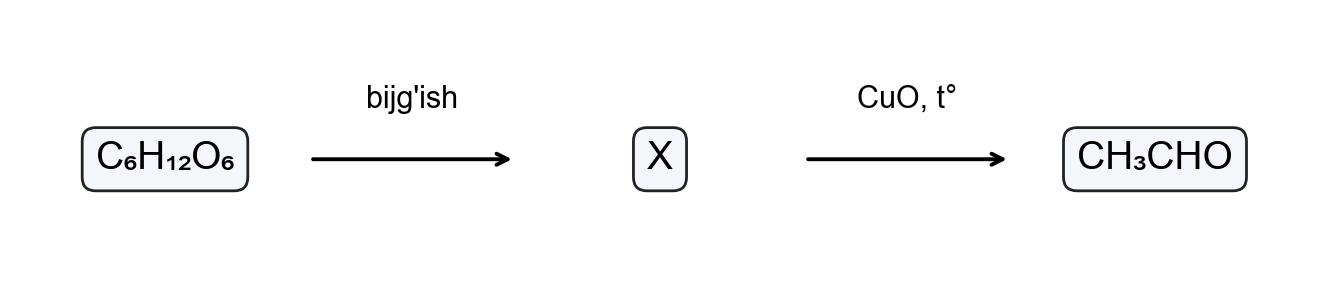
\includegraphics[width=0.86\linewidth]{rasmlar/gen/co_301396.png}\end{center}

\noindent A)~\textsl{C\textsubscript{2}H\textsubscript{5}ONa} \hfill B)~\textsl{CH\textsubscript{3}COONa} \hfill C)~\textsl{CH\textsubscript{3}CHO} \hfill D)~\textsl{C\textsubscript{2}H\textsubscript{5}OH}\par
\qsep
\noindent\qn{24.} Benzol va toluol aralashmasi yondirilganda 3,2 mol CO\textsubscript{2} va 1,7 mol suv hosil bo`ldi. Aralashmadagi benzolning mol \textbf{ulushini (\%) aniqlang.}

\noindent A)~\textsl{40} \hfill B)~\textsl{60} \hfill C)~\textsl{56} \hfill D)~\textsl{50}\par
\qsep
\noindent\qn{25.} Metilformiat va metilatsetat aralashmasi (28,2 g) mo`l NaOH eritmasi bilan to`liq gidrolizlandi. Aralashmaning mol miqdori 0,4 mol. Hosil bo`lgan spirtlar \textbf{massasini (g) aniqlang.}

\noindent A)~\textsl{25,6} \hfill B)~\textsl{12,8} \hfill C)~\textsl{15,4} \hfill D)~\textsl{6,4}\par
\qsep
\noindent\qn{26.} 324 g kraxmal gidrolizlanib (unum 90\%) glukoza olindi, glukoza esa spirtli bijg`ishga uchradi (unum 60\%). Hosil bo`lgan etanol \textbf{massasini (g) toping.}

\noindent A)~\textsl{49,7} \hfill B)~\textsl{198,7} \hfill C)~\textsl{165,6} \hfill D)~\textsl{99,4}\par
\qsep
\noindent\qn{27.} C\textsubscript{6}H\textsubscript{5}NO\textsubscript{2} dan quyidagi sxema bo`yicha 25,9 g fenilammoniy xlorid olindi: C\textsubscript{6}H\textsubscript{5}NO\textsubscript{2} $\to$ C\textsubscript{6}H\textsubscript{5}NH\textsubscript{2} $\to$ [C\textsubscript{6}H\textsubscript{5}NH\textsubscript{3}]Cl. Bosqichlarning unumi ketma-ket 40\%, 50\% ni tashkil qiladi. Barcha reaksiyalar 1 atm bosimda olib borildi. Sarflangan C\textsubscript{6}H\textsubscript{5}NO\textsubscript{2} massasi (g) \textbf{ni aniqlang.}

\noindent A)~\textsl{246} \hfill B)~\textsl{123} \hfill C)~\textsl{61,5} \hfill D)~\textsl{49,2}\par
\qsep
\noindent\qn{28.} C\textsubscript{2}H\textsubscript{4} dan quyidagi sxema bo`yicha 26,01 g sirka kislota olindi: C\textsubscript{2}H\textsubscript{4} $\to$ C\textsubscript{2}H\textsubscript{5}OH $\to$ CH\textsubscript{3}CHO $\to$ CH\textsubscript{3}COOH. Bosqichlarning unumi ketma-ket 85\%, 60\%, 85\% ni tashkil qiladi. Sarflangan C\textsubscript{2}H\textsubscript{4} hajmi (l, n.sh.) \textbf{ni aniqlang.}

\noindent A)~\textsl{22,4} \hfill B)~\textsl{44,8} \hfill C)~\textsl{11,2} \hfill D)~\textsl{19,04}\par
\qsep
\noindent\qn{29.} 448 l (n.sh.) C\textsubscript{3}H\textsubscript{6} dan quyidagi sxema bo`yicha aseton olindi: CH\textsubscript{3}--CH=CH\textsubscript{2} $\to$ CH\textsubscript{3}--CHCl--CH\textsubscript{3} $\to$ CH\textsubscript{3}--CH(OH)--CH\textsubscript{3} $\to$ CH\textsubscript{3}--CO--CH\textsubscript{3}. Bosqichlarning unumi ketma-ket 50\%, 60\%, 85\% ni tashkil qiladi. Barcha reaksiyalar 1 atm bosimda olib borildi. Olingan aseton \textbf{massasini (g) aniqlang.}

\noindent A)~\textsl{591,6} \hfill B)~\textsl{295,8} \hfill C)~\textsl{147,9} \hfill D)~\textsl{348}\par
\qsep
\noindent\qn{30.} Laboratoriyada olingan xlor qanday usulda yig`iladi?
\noindent A)~\textsl{havoni siqib chiqarish (idish og`zi pastga)}\par
\noindent B)~\textsl{suvni siqib chiqarish usulida}\par
\noindent C)~\textsl{gazni suyuqlantirib yig`iladi}\par
\noindent D)~\textsl{havoni siqib chiqarish (idish og`zi yuqoriga)}\par
\qsep
\noindent\qn{31.} Quyidagi jarayonlar qanday kuzatuvlar bilan boradi? To`g`ri ta'riflangan \textbf{jarayonlarni belgilang.} 1) NaOH eritmasiga CuSO\textsubscript{4} eritmasi tomchilab qo`shilganda (ishqor mo`l): ko`k cho`kma tushadi, keyin ko`k cho`kma hosil bo`ladi va erimaydi; 2) FeCl\textsubscript{3} eritmasiga avval NaOH, so`ng mo`l HCl eritmasi qo`shilganda: qo`ng`ir-qizil cho`kma tushadi, keyin cho`kma erimasdan qoladi; 3) CuSO\textsubscript{4} eritmasiga avval NaOH, so`ng mo`l ammiak eritmasi qo`shilganda: ko`k cho`kma tushadi, keyin cho`kma qo`ng`ir tusga kiradi; 4) ZnSO\textsubscript{4} eritmasiga avval oz, so`ng mo`l NaOH eritmasi qo`shilganda: oq cho`kma tushadi, keyin cho`kma erimasdan qoladi

\noindent A)~\textsl{1} \hfill B)~\textsl{1, 3} \hfill C)~\textsl{3, 4} \hfill D)~\textsl{1, 4}\par
\qsep
\noindent\qn{32.} Rasmdagi asbob bilan qaysi aralashmani ajratish mumkin?
\begin{center}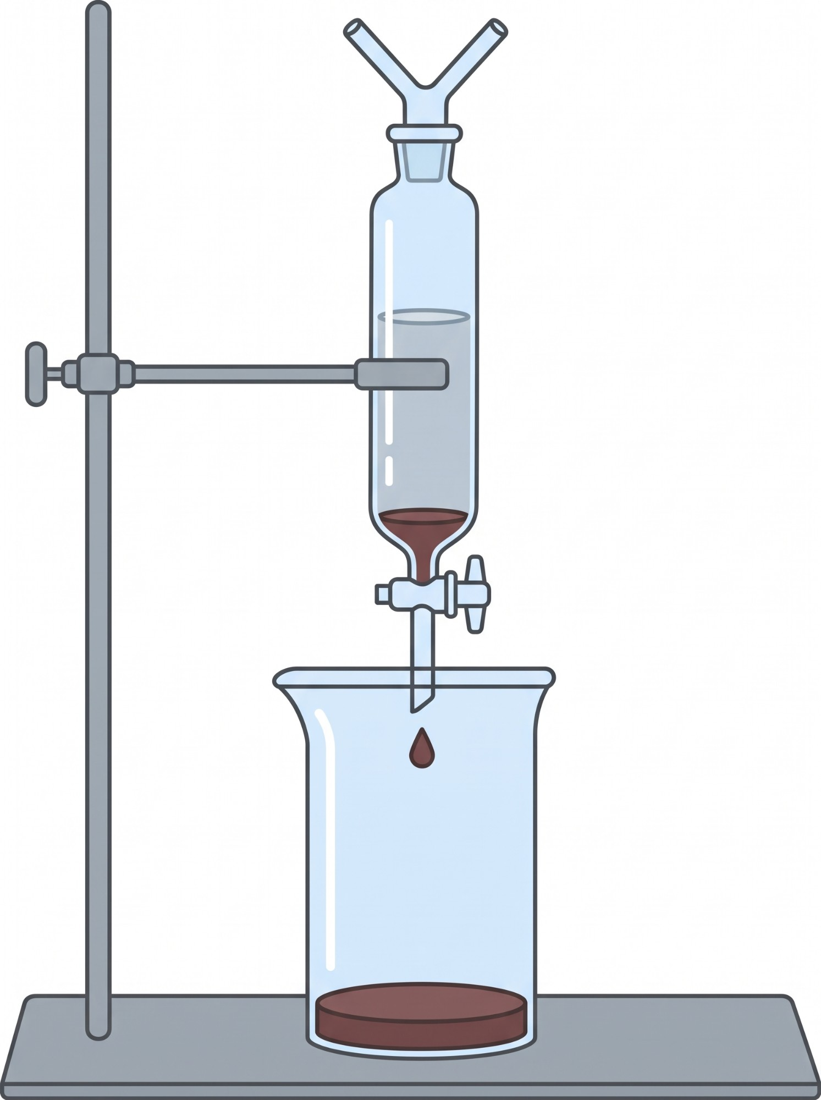
\includegraphics[width=0.86\linewidth]{rasmlar/darslik/d_ajratgich.png}\end{center}

\noindent\begin{tabular}{@{}p{0.47\linewidth}@{}p{0.47\linewidth}@{}}
A)~\textsl{suv va qum} & B)~\textsl{suv va etanol} \\
C)~\textsl{osh tuzi eritmasi} & D)~\textsl{suv va kerosin   ---} \\
\end{tabular}\par
\qsep
\end{multicols}
\medskip
\noindent\setlength{\fboxsep}{0pt}\fbox{\begin{tabular}{p{0.74\linewidth}|p{0.2\linewidth}}
\parbox[t]{0.72\linewidth}{\vspace{3pt}\textbf{Topshiriqlar (33--35) va javob variant (A--F)larini o`zaro to`g`ri moslashtiring.} 1,88 g CuSO\textsubscript{4}$\cdot$5H\textsubscript{2}O suvda eritilib, hajmi 500 ml bo`lgan eritma tayyorlandi. Eritma inert elektrodlar yordamida 5 A tok kuchi bilan 96 s elektroliz qilindi (eritma hajmi o`zgarmadi deb hisoblang). Elektrolizdan keyin eritmaga mo`l NaOH qo`shilib, hosil bo`lgan cho`kma ajratildi, qizdirildi, so`ng hosil bo`lgan qattiq modda vodorod oqimida to`liq qaytarildi.
\vspace{3pt}} & \parbox[t]{0.19\linewidth}{\vspace{3pt}A~\textsl{0,64}\\[3pt]
B~\textsl{0,32}\\[3pt]
C~\textsl{2}\\[3pt]
D~\textsl{0,26}\\[3pt]
E~\textsl{1,6}\\[3pt]
F~\textsl{0,01}}\\ \hline
\parbox[t]{0.72\linewidth}{\vspace{2pt}\textbf{33. Dastlabki eritmada CuSO\textsubscript{4} ning molyar konsentratsiyasini (mol/l) hisoblang.}\vspace{2pt}} & \\ \hline
\parbox[t]{0.72\linewidth}{\vspace{2pt}\textbf{34. Elektroliz tugagach eritmaning pH ini aniqlang.}\vspace{2pt}} & \\ \hline
\parbox[t]{0.72\linewidth}{\vspace{2pt}\textbf{35. Oxirida olingan metall massasini (g) toping.}\vspace{2pt}} & 
\end{tabular}}
\par\bigskip
\noindent\qn{36.} 25\% li va 5\% li tuz eritmalari massalar nisbati 3 : 2 bo`lgan holda aralashtirildi. Tajriba 10 daqiqa davom etdi. Hosil bo`lgan eritmaning massa \textbf{ulushini (\%) hisoblang.}
\javob\qsep
\noindent\qn{37.} Reaksiya 30 \textdegree{}C da 72 minutda tugaydi. $\gamma$ = 2. Harorat 30 \textdegree{}C ga oshirilib, reagentlardan birining konsentratsiyasi 2 marta oshirildi (reaksiya shu modda bo`yicha 1-tartibli). Tajriba hajmi 250 ml bo`lgan kolbada o`tkazildi. Reaksiya necha minutda tugaydi?
\javob\qsep
\noindent\qn{38.} 2SO\textsubscript{3} $\rightleftarrows$ 2SO\textsubscript{2} + O\textsubscript{2} reaksiyasi doimiy harorat va bosimda olib borildi; boshlang`ich modda qisman o`zgargach gazlar hajmi 11/8 marta ortdi. Tajriba laboratoriyada, chinni idishda o`tkazildi. Boshlang`ich modda necha foizi \textbf{o`zgarganini aniqlang.}
\javob\qsep
\noindent\qn{39.} Bir atomli to`yingan noma'lum spirtning 18,4 g miqdori natriy bilan ta'sirlashganda 4,48 l (n.sh.) vodorod ajraldi. Shu spirtning 1/2 qismi mis(II) oksid bilan oksidlandi, hosil bo`lgan modda mo`l ammiakli kumush oksid eritmasi bilan qizdirildi. Ajralgan kumush \textbf{massasini (g) toping.}
\javob\qsep
\noindent\qn{40.} Bir asosli to`yingan karbon kislotaning 22,2 g miqdori mo`l NaHCO\textsubscript{3} bilan ta'sirlashganda 6,72 l (n.sh.) gaz ajraldi. Shu kislotaning 2/3 qismi mo`l etanol bilan esterlandi (efir unumi 4/5). Hosil bo`lgan murakkab efirning \textbf{massasini (g) toping.}
\javob\qsep
\par\bigskip\begin{center}\textbf{\fontsize{13}{15}\selectfont YOZMA ISH}\end{center}
\noindent\qn{41.} \textbf{Topshiriqni bajarish jarayonida barcha reaksiya tenglamalarini yozing. Miqdoriy va arifmetik hisoblashlarni (unga asos bo`lgan usul yoki formulani ko`rsatgan holda) uzviy ketma-ketlikda bajaring.}\par\smallskip
Tarkibi XSO\textsubscript{4}$\cdot$nH2O bo`lgan (\textit{X} -- oksidlanish darajasi +2 bo`lgan metall) kristallogidratning 12,5 g namunasida suvning massa ulushi 36\% ni tashkil etadi. Namuna suvda eritilib, mo`l BaCl\textsubscript{2} eritmasi qo`shilganda 11,65 g cho`kma tushdi. Reagent (BaCl\textsubscript{2}) eritmasining massa ulushi 50\% va zichligi 1,05 g/ml; u mo`l miqdorda olingan. Cho`kma ajratilgach, filtratga mo`l NaOH eritmasi qo`shilib, hosil bo`lgan gidroksid doimiy massagacha kuydirildi.\par
\noindent 1)\ Barcha reaksiyalarning tenglamalarini yozing; kristallogidratning molyar massasini va tuzdagi (suvsiz) qismining molyar massasini hisoblang.\par
\noindent 2)\ \textit{X} metallni aniqlang va n ning qiymatini toping.\par
\noindent 3)\ Namunadagi XSO\textsubscript{4} ning (suvsiz) massasini va kristallizatsion suv massasini (g) hisoblang.\par
\noindent 4)\ Filtratga sarflangan NaOH ning minimal miqdorini (mol) toping.\par
\noindent 5)\ Kuydirishdan hosil bo`lgan oksid massasini (g) aniqlang va u namuna massasining necha foizini tashkil etishini toping.\par
\diqqat{Mazkur topshiriq kengaytirilgan javobni talab etib, uning yechilish usuli va shu usul asosidagi barcha hisoblash amallari javoblar varaqasida aks etishi lozim.}\qsep
\noindent\qn{42.} Organik moddalarning xossalarini bilgan holda reaksiya tenglamalarini tugallang va tenglashtiring. 3- va 5-reaksiyalarda hosil bo`lgan asosiy organik mahsulotlarni sistematik nomenklatura bo`yicha nomlang. Hosil bo`lgan organik moddalarning tuzilish formulalarini yozing.\par
\noindent 1)\ CH$\equiv$CH + H\textsubscript{2}O (Hg\textsuperscript{2+}, H\textsuperscript{+}) $\to$\par
\noindent 2)\ CH\textsubscript{3}--CH\textsubscript{2}--OH + CH\textsubscript{3}--COOH (H\textsubscript{2}SO\textsubscript{4}, t) $\rightleftarrows$\par
\noindent 3)\ CH\textsubscript{3}--CH\textsubscript{2}--OH (H\textsubscript{2}SO\textsubscript{4} kons., 170 \textdegree{}C) $\to$\par
\noindent 4)\ 2CH\textsubscript{3}--CH\textsubscript{2}--OH (H\textsubscript{2}SO\textsubscript{4} kons., 140 \textdegree{}C) $\to$\par
\noindent 5)\ C\textsubscript{6}H\textsubscript{6} + HNO\textsubscript{3} (H\textsubscript{2}SO\textsubscript{4} kons., t) $\to$\par
\noindent 6)\ C\textsubscript{6}H\textsubscript{5}--CH\textsubscript{3} + Cl\textsubscript{2} (yorug`lik) $\to$\par
\noindent 7)\ CH\textsubscript{3}--CHO + H\textsubscript{2} (Ni, t) $\to$\par
\diqqat{Mazkur topshiriq kengaytirilgan javobni talab etib, uning yechilish usuli va shu usul asosidagi barcha hisoblash amallari javoblar varaqasida aks etishi lozim.}\qsep
\noindent\qn{43.} \textbf{Topshiriqni bajarish jarayonida barcha reaksiya tenglamalarini yozing. Miqdoriy va arifmetik hisoblashlarni (unga asos bo`lgan usul yoki formulani ko`rsatgan holda) uzviy ketma-ketlikda bajaring.}\par\smallskip
Tarkibida AgNO\textsubscript{3} va Cu(NO\textsubscript{3})\textsubscript{2} bo`lgan 300 g eritmaga temir plastinka tushirildi (Ag\textsuperscript{+} va Cu\textsuperscript{2+} ning hammasi o`rnini bosdi). Plastinkada ajralgan metallar massasi 28 g, plastinka massasi esa 16,8 g ga ortdi. Plastinka olingach, eritmaga mo`l NaOH eritmasi qo`shildi, hosil bo`lgan cho`kma havoda to`liq oksidlanib, so`ng doimiy massagacha kuydirildi. Reagent (NaOH) eritmasining massa ulushi 10\% va zichligi 1,4 g/ml; u mo`l miqdorda olingan. Kuydirishdan hosil bo`lgan oksid alyuminiy bilan qizdirilganda (alyuminotermiya) metall hosil bo`ldi; bu metall mo`l xlorid kislotada eritilib, ajralgan gaz qizdirilgan mis(II) oksid ustidan o`tkazildi.\par
\noindent 1)\ Barcha reaksiyalarning tenglamalarini yozing va tenglashtiring. Eritmadagi AgNO\textsubscript{3} va Cu(NO\textsubscript{3})\textsubscript{2} ning miqdorlarini (mol) toping.\par
\noindent 2)\ Eritmaga o`tgan temirning massasini (g) hisoblang.\par
\noindent 3)\ Plastinka olingandan keyin eritmadagi Fe(NO\textsubscript{3})\textsubscript{2} ning massa ulushini (\%) aniqlang. Alyuminotermiyada sarflangan alyuminiy massasini (g) hisoblang.\par
\noindent 4)\ Cho`kmani oksidlashga sarflangan kislorodning hajmini (l, n.sh.) hisoblang. Metallning xlorid kislota bilan reaksiyasida ajralgan gaz hajmini (l, n.sh.) toping.\par
\noindent 5)\ Kuydirishdan hosil bo`lgan qattiq moddaning massasini (g) toping. Gaz mis(II) oksid bilan reaksiyaga kirishganda hosil bo`lgan mis massasini (g) aniqlang.\par
\diqqat{Mazkur topshiriq kengaytirilgan javobni talab etib, uning yechilish usuli va shu usul asosidagi barcha hisoblash amallari javoblar varaqasida aks etishi lozim.}\qsep
\newpage
\noindent\textbf{\fontsize{13}{15}\selectfont 3-variant}\hfill \textbf{Javoblar kaliti}\par\smallskip\hrule\smallskip
\textit{Faqat o`qituvchi uchun.}\par\medskip
\noindent\textbf{1--32-savollar}\par\smallskip
\noindent\begin{tabular}{|c|c|c|c|c|c|c|c|c|c|c|c|c|c|c|c|}\hline
\textbf{1} & \textbf{2} & \textbf{3} & \textbf{4} & \textbf{5} & \textbf{6} & \textbf{7} & \textbf{8} & \textbf{9} & \textbf{10} & \textbf{11} & \textbf{12} & \textbf{13} & \textbf{14} & \textbf{15} & \textbf{16}\\\hline
\textsl{C} & \textsl{C} & \textsl{B} & \textsl{B} & \textsl{A} & \textsl{A} & \textsl{C} & \textsl{D} & \textsl{D} & \textsl{A} & \textsl{C} & \textsl{C} & \textsl{C} & \textsl{B} & \textsl{B} & \textsl{A}\\\hline
\textbf{17} & \textbf{18} & \textbf{19} & \textbf{20} & \textbf{21} & \textbf{22} & \textbf{23} & \textbf{24} & \textbf{25} & \textbf{26} & \textbf{27} & \textbf{28} & \textbf{29} & \textbf{30} & \textbf{31} & \textbf{32}\\\hline
\textsl{A} & \textsl{D} & \textsl{A} & \textsl{C} & \textsl{C} & \textsl{D} & \textsl{D} & \textsl{B} & \textsl{B} & \textsl{D} & \textsl{B} & \textsl{A} & \textsl{B} & \textsl{D} & \textsl{A} & \textsl{D}\\\hline
\end{tabular}\par\medskip
\noindent\textbf{33--35-savollar}\par\smallskip
\noindent\begin{tabular}{|c|c|c|}\hline \textbf{No} & \textbf{Javob} & \textbf{Qiymat}\\\hline
33 & \textsl{F} & 0,01\\\hline
34 & \textsl{C} & 2\\\hline
35 & \textsl{B} & 0,32\\\hline
\end{tabular}\par\medskip
\noindent\textbf{36--40-savollar}\par\smallskip
\noindent\begin{tabular}{|c|c|}\hline \textbf{No} & \textbf{To`g`ri javob}\\\hline
36 & 17\\\hline
37 & 4,5\\\hline
38 & 75\\\hline
39 & 43,2\\\hline
40 & 16,32\\\hline
\end{tabular}\par\medskip
\noindent\textbf{41--43-topshiriqlar: javoblar}\par\smallskip
\noindent\textbf{41-topshiriq.}\par
\noindent 1) 250 g/mol; 160 g/mol\par
\noindent 2) Cu; 5\par
\noindent 3) 8 g; 4,5 g\par
\noindent 4) 0,1 mol\par
\noindent 5) 4 g; 32\%\par
\noindent\textbf{42-topshiriq.}\par
\noindent 1) CH$\equiv$CH + H\textsubscript{2}O $\to$ CH\textsubscript{3}--CHO\par
\noindent 2) CH\textsubscript{3}--CH\textsubscript{2}--OH + CH\textsubscript{3}--COOH $\rightleftarrows$ CH\textsubscript{3}--COO--CH\textsubscript{2}--CH\textsubscript{3} + H\textsubscript{2}O\par
\noindent 3) CH\textsubscript{3}--CH\textsubscript{2}--OH $\to$ CH\textsubscript{2}=CH\textsubscript{2} + H\textsubscript{2}O --- nomi: \textbf{etilen}\par
\noindent 4) 2CH\textsubscript{3}--CH\textsubscript{2}--OH $\to$ CH\textsubscript{3}--CH\textsubscript{2}--O--CH\textsubscript{2}--CH\textsubscript{3} + H\textsubscript{2}O\par
\noindent 5) C\textsubscript{6}H\textsubscript{6} + HNO\textsubscript{3} $\to$ C\textsubscript{6}H\textsubscript{5}--NO\textsubscript{2} + H\textsubscript{2}O --- nomi: \textbf{nitrobenzol}\par
\noindent 6) C\textsubscript{6}H\textsubscript{5}--CH\textsubscript{3} + Cl\textsubscript{2} $\to$ C\textsubscript{6}H\textsubscript{5}--CH\textsubscript{2}Cl + HCl\par
\noindent 7) CH\textsubscript{3}--CHO + H\textsubscript{2} $\to$ CH\textsubscript{3}--CH\textsubscript{2}--OH\par
\noindent\textbf{43-topshiriq.}\par
\noindent 1) 0,2 mol; 0,1 mol\par
\noindent 2) 11,2 g\par
\noindent 3) 12,71\%; 5,4 g\par
\noindent 4) 1,12 l; 4,48 l\par
\noindent 5) 16 g; 12,8 g\par
\par\bigskip\noindent\textbf{Mavzular taqsimoti}\par\smallskip
{\small\noindent\begin{longtable}{|c|p{7.2cm}|p{5.4cm}|c|}\hline \textbf{No} & \textbf{Mavzu} & \textbf{Tekshiriladigan ko`nikma} & \textbf{Ball}\\\hline
1 & Tirkashev I bob (kvant sonlari) & Bilim va tushunish & 1\\\hline
2 & Tirkashev I bob; 8-sinf (izoelektron) & Bilim va tushunish & 1\\\hline
3 & 11-sinf 8-bob; Tirkashev \textit{V} bob (elektroliz) & Bilim va tushunish & 1\\\hline
4 & Tirkashev \textit{V} bob; 11-sinf 7-bob (OQR tenglash) & Hisoblash va masala yechish & 1\\\hline
5 & 9-sinf; 11-sinf (pH; neytrallanish) & Hisoblash va masala yechish & 1\\\hline
6 & Tirkashev VI bob (reaksiya tezligi, grafik) & Grafik tahlili & 1\\\hline
7 & 9-sinf (kalsiy birikmalari; mantiqiy masala) & Hisoblash va masala yechish & 1\\\hline
8 & 8-10-sinf ($\sigma$- va $\pi$-bog`lar) & Hisoblash va masala yechish & 1\\\hline
9 & 9-sinf (elektrolitik dissotsilanish) & Hisoblash va masala yechish & 1\\\hline
10 & Tirkashev VI bob (muvozanat, jadval) & Jadval tahlili & 1\\\hline
11 & Tirkashev VI bob (muvozanat, jadval) & Jadval tahlili & 1\\\hline
12 & Tirkashev VI bob (Le-Shatelye) & Bilim va tushunish & 1\\\hline
13 & Tirkashev VI bob; 11-sinf (muvozanat) & Hisoblash va masala yechish & 1\\\hline
14 & Tashev (nitratlar) & Bilim va tushunish & 1\\\hline
15 & 8-sinf; 9-sinf (genetik bog`lanish) & Bilim va tushunish & 1\\\hline
16 & 9-sinf (amfoter oksidlar) & Hisoblash va masala yechish & 1\\\hline
17 & 9-sinf; Tirkashev (suv qattiqligi, hisob) & Hisoblash va masala yechish & 1\\\hline
18 & 9-11-sinf (gaz hajmi o`zgarishi; parchalanish darajasi) & Hisoblash va masala yechish & 1\\\hline
19 & 9-sinf (mineral o`g`itlar) & Hisoblash va masala yechish & 1\\\hline
20 & 10-sinf \S{}6, \S{}12, \S{}20, \S{}28 (izomeriya) & Bilim va tushunish & 1\\\hline
21 & 10-sinf (mavzuga oid paragraflar); Abdusamatov & Bilim va tushunish & 1\\\hline
22 & 10-sinf (spirt, aldegid, fenol sifat reaksiyalari) & Bilim va tushunish & 1\\\hline
23 & 10-sinf (organik moddalarning o`zaro bog`lanishi) & Rasm bo`yicha tahlil & 1\\\hline
24 & 10-sinf (arenlar; yonish) & Hisoblash va masala yechish & 1\\\hline
25 & 10-sinf (murakkab efirlarning gidrolizi) & Hisoblash va masala yechish & 1\\\hline
26 & 10-sinf (uglevodlar: kraxmal, glukoza) & Hisoblash va masala yechish & 1\\\hline
27 & 10-sinf (nitrobirikmalar, aminlar) & Hisoblash va masala yechish & 1\\\hline
28 & 10-sinf (alkenlar, spirtlar, aldegidlar, kislotalar) & Hisoblash va masala yechish & 1\\\hline
29 & 10-sinf (alkenlar, galogenli hosilalar, spirtlar) & Hisoblash va masala yechish & 1\\\hline
30 & 9--10-sinf (gazlarni yig`ish) & Bilim va tushunish & 1\\\hline
31 & 9-sinf; 11-sinf (amfoter birikmalar, kompleks hosil bo`lishi) & Bilim va tushunish & 1\\\hline
32 & 7-sinf (10-rasm) & Rasm bo`yicha tahlil & 1\\\hline
33--35 & Aralash masala (moslashtirish) & Ko`p bosqichli hisob & 3\\\hline
36--40 & Qisqa javobli masalalar & Hisoblash & 5\\\hline
41--43 & Yozma ish & Usul va hisob (M, A) & 75\\\hline
\end{longtable}}
\end{document}
